\section{Serial Version}

\begin{frame}{Serial Version}
    The Huffman Compression Algorithm is composed by four phases:
    \begin{enumerate}
        \item Count the byte frequencies
        \item Build the Huffman tree using the frequencies
        \item Generate the Huffman alphabet by visiting the Huffman tree by using a DFS algorithm
        \item Data encoding using the Huffman alphabet
    \end{enumerate}
\end{frame}

\begin{frame}{Build the Huffman Tree}
    \centering
    \scalebox{.8}{
        \begin{algorithm}[H]
            \caption{Build the Huffman tree}\label{alg:buildtree}
            \SetKwData{Q}{Q}\SetKwData{z1}{z1}\SetKwData{z2}{z2}\SetKwData{z}{z}
            \SetKwFunction{insert}{insert}\SetKwFunction{deleteMin}{deleteMin}
            \SetKwInOut{Input}{input}\SetKwInOut{Output}{output}
            \SetKwFor{}{}{}{}
            // Populate the min priority queue with characters and their frequencies\;
            \For{\(i=1\) \KwTo \(n-1\)}{
                Q.insert(f[i], Tree(f[i], c[i]))\;
            }
            // Repeat until the queue has only a single element left\;
            \For{\(i=1\) \KwTo \(n-1\)}{
                // Get the two least frequent nodes\;
                z1, z2 = Q.deleteMin(), Q.deleteMin()\;
                // Create and insert inner tree node into the queue\;
                z = Tree(z1.f + z2.f, null)\;
                z.left, z.right = z1, z2\;
                Q.insert(z.f, z)\;
            }
            // The last element in the queue is the root of the Huffman tree\;
            \Return{Q.deleteMin()}\;
        \end{algorithm}
    }
\end{frame}

\begin{frame}{Get the Huffman Alphabet from the Tree}
    Make a DFS visit of the Tree from root to leaves
    \begin{center}
        \begin{figure}[h!]
            \centering
            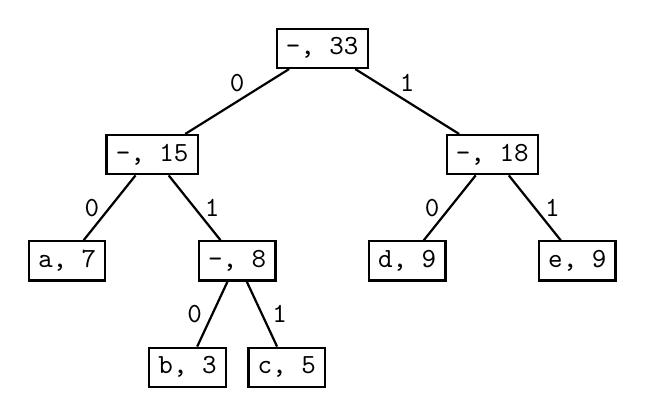
\begin{tikzpicture}
                [
                    level distance=1.5cm,
                    level 1/.style={sibling distance=4.8cm},
                    level 2/.style={sibling distance=2.4cm},
                    level 3/.style={sibling distance=1.4cm},
                    thick,
                    font=\ttfamily\bfseries, scale=0.9
                ]
                \tikzset{
                    treenode/.style = {rectangle, draw=black, align=center,minimum width=0.75cm},
                    edgestyleL/.style = {midway,left,draw=none},
                    edgestyleR/.style = {midway,right,draw=none}
                }
                \node [treenode] (T) {-, 33}
                child { node[treenode] (L) {-, 15}
                        child { node[treenode] (LL) {a, 7} edge from parent node[edgestyleL] {0} }
                        child { node[treenode] (LR) {-, 8}
                                child { node[treenode] (LRL) {b, 3} edge from parent node[edgestyleL] {0} }
                                child { node[treenode] (LRR) {c, 5} edge from parent node[edgestyleR] {1} }
                                edge from parent node[edgestyleR] {1}
                            }
                        edge from parent node[edgestyleL,above] {0}
                    }
                child { node[treenode] (R) {-, 18}
                        child { node[treenode] {d, 9} edge from parent node[edgestyleL] {0}}
                        child { node[treenode] {e, 9} edge from parent node[edgestyleR] {1}}
                        edge from parent node[edgestyleR,above] {1}
                    }
                ;
            \end{tikzpicture}
            \caption{An example of Huffman tree.}
            \label{fig:tree}
        \end{figure}
    \end{center}
\end{frame}


